\newpage	
\section{Reconocimiento de texto en escenas naturales}

	En el capítulo anterior, se desarrollaron los conceptos necesarios para entender las bases del aprendizaje supervisado y los clasificadores probabilísticos. Todos estos conceptos sirven para entender los principios sobre los que se asienta el trabajo realizado por Wang et. al. en \cite{wang}. El trabajo de los autores, abarca el reconocimiento de texto en escenas naturales en todas sus etapas. En particular, una de ellas es el reconocimiento de caracteres.
	
	En este capitulo se van a presentar dos implementaciones: la provista originalmente por Wang et al. en \cite{wang} y la realizada en este trabajo basándose en la primera. Solamente se van a desarrollar los temas referentes al reconocimiento de caracteres ya que el presente trabajo se enfoca únicamente en ese problema.
	
	
	\subsection{Introducción}

	En el trabajo que realizaron Wang et al., los autores identificador el problema que había al detectar y reconocer palabras en imágenes naturales. Ellos identifican, que si bien las actuales aplicaciones de OCR se manejan bien con documentos escaneados, todavía encuentran problemas cuando tratan de procesar texto adquirido en entornos naturales (también referido como texto de escena). Este tipo de texto se ha vuelto más frecuente debido al aumento de dispositivos que son capaces de extraer dicha información, sean estos celulares, tabletas o cámaras.
	
	Durante la competencia de ICDAR (\textit{International Conference on Document Analysis and Recognition}) en 2003, los organizadores tenían como objetivo ver cual era el estado del arte en las diferentes etapas del reconocimiento de texto en escenas naturales. Observaron que habían imágenes con texto que los motores de OCR del momento no podían procesar, por lo tanto, decidieron dividir el problema general que era reconocer palabras en escenas naturales en tres subproblemas:
	
	\begin{itemize}
		\item \textbf{La clasificación de caracteres recortados.}
		
		En este problema se consideran imagenes de caracteres extraidas de escenas naturales. Las imagenes contienen exclusivamente un sólo carácter y sus tamaños se ajustan a las dimensiones del caracter tal como se puede apreciar en la Figura \ref{fig: Caracteres recortados}. El objetivo es identificar qué carácter está reflejado en la imagen a partir de un conjunto predefinido de caracteres que hacen al problema.

		Una de las dificultades de este problema es que algunos caracteres son muy difíciles de dicernir entre sí, por ejemplo, si consideramos las letras mayúsculas y las minúsculas por separado, luego una ``Z'' es muy difícil de dicernir de una ``z''. Incluso se puede dar lugar a la confusión entre distintos símbolos, por ejemplo, la ``O'' (letra o mayúscula) y el número ``0'' o el número ``6'' y la ``G'' (letra ``g'' mayúscula).
						
		Otro elemento que se tiene que tener presente al momento de clasificar caracteres, es el tipo de características locales que se van a obtener de cada imagen. Como se ha explicado en la sección \ref{subsection:feature}, las características son importantes dado que representa los aspectos o cualidades más significativas de un objeto. Si se hace una buena elección de las características locales, se va a ver reflejado en la performance de clasificación.
		
		Las condiciones en que fueron tomadas las imágenes donde se extrajeron los caracteres influye posteriormente en su reconocimiento. Por ejemplo, las variaciones en las condiciones de iluminación, oclusión, posicionamiento al momento de tomar la imagen, etc. Para resolver esto, se puede realizar un pre-procesamiento que ayude a ``limpiar'' la imagen para poder facilitar su reconocimiento posterior.
		
	\begin{figure}[htbp]
		\centering
  		\centerline{ 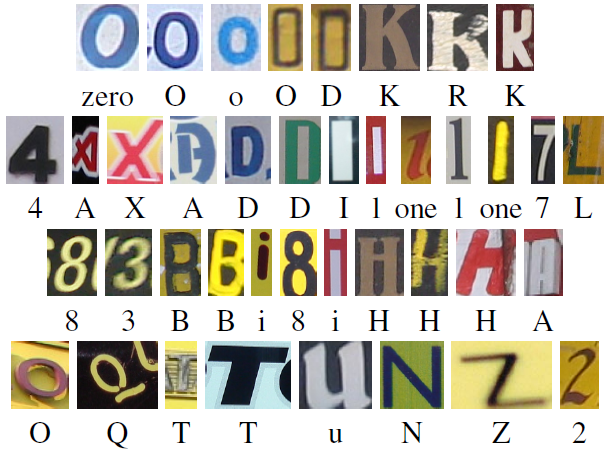
\includegraphics[scale=0.5]{img/hog/confusing_english.png} }
		\caption[Clasificación de caracteres recortados]{Conjunto de caracteres recortados. Imagen extraida del paper de T. E. de Campos et. al. \cite{dCBV09}}
		\label{fig: Caracteres recortados}
	\end{figure}
		
		\item \textbf{Detección de zonas con texto en la imagen.}
		
		Este problema involucra la detección de zonas de la imagen que pueden contener texto. Esto se realiza con el objetivo de priorizar estas regiones en procesamientos posteriores para reducir la complejidad del problema del análisis de texto. La figura \ref{fig: Zona texto} expone un ejemplo de este problema.
		
		Para poder resolver este problema, se debe considerar que las palabras que conforman el texto a detectar, pueden haber sido adquiridas a distintas escalas. Tal es el caso del texto de casi la mayoría de los carteles publicitarios que es posible encontrar en las calles de una ciudad. Otro factor a considerar es la inclinación del texto que puede darse por la posición del observador. Además, esta tarea se dificulta si consideramos, al igual que en el reconocimiento de caracteres, las condiciones de la imagen (iluminación, distorsiones, estilo y fuente de las palabras en el texto, etc).
		
		En el trabajo de Chen H. et. al. \cite{ChenH11}, los autores destacan que hay dos categorías al momento de diferenciar las técnicas de reconocimiento de texto. La primera categoría, son las técnicas \textit{basadas en textura} (\textit{texture based} de su traducción al inglés) que destacan al texto como una ``textura'' especial que es distinguible del fondo. Las características se extraen de ciertas regiones de la imagen y se utiliza un clasificador para identificar la existencia de texto. La segunda categoría, son las técnicas basadas en \textit{componentes conectados} (\textit{connected component} de su traducción al inglés), donde se extraen regiones de la imagen y se utilizan restricciones geométricas para descartar candidatos que no sean texto.
		
	\begin{figure}[htbp]
		\centering
		\centerline{ 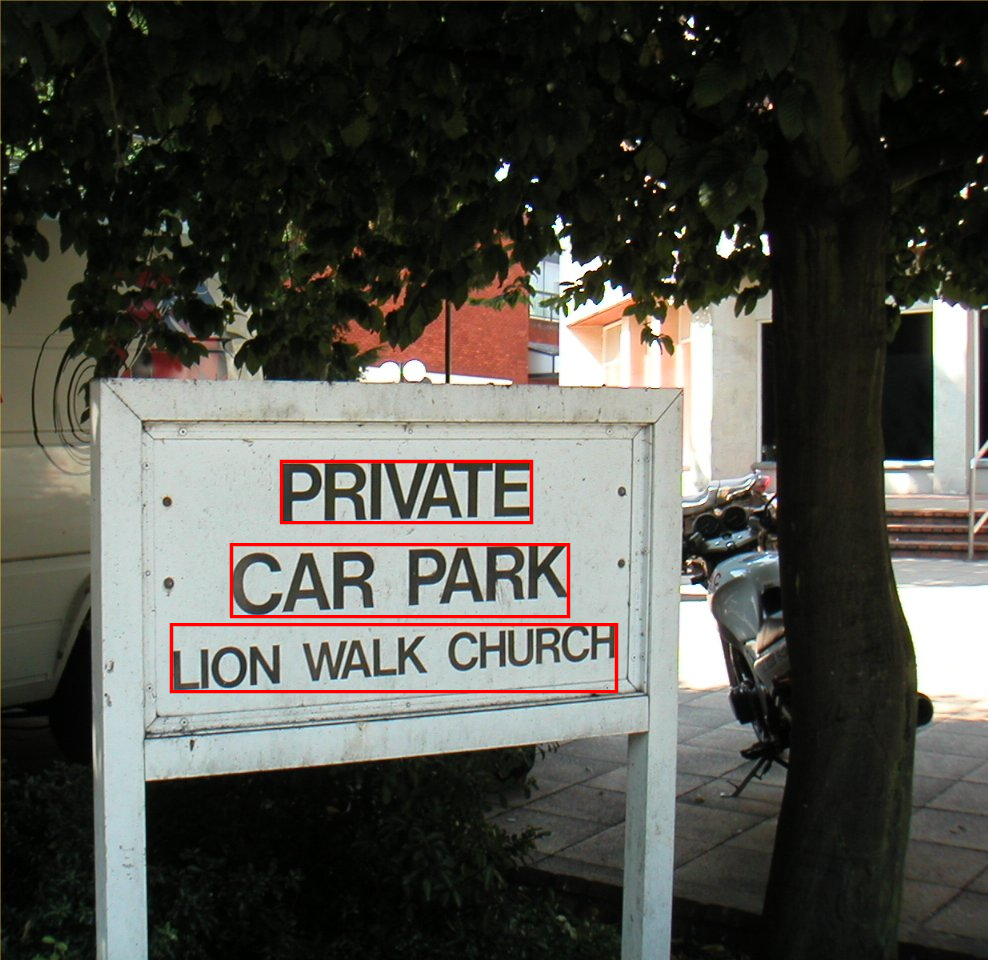
\includegraphics[scale=0.20]{img/zone_with_text.png} }
		\caption[Detección de zonas con texto]{Imagen natural donde las zonas con texto están encasilladas.Imagen tomada del sitio \url{http://libccv.org/post/introducing-ccv-milestone/} }
		\label{fig: Zona texto}
	\end{figure} 
		
		\item \textbf{El reconocimiento de palabras recortadas.}

		En este problema se busca identificar las palabras que se encuentran dentro de las imágenes recortadas. Al igual que el problema del reconocimiento de caracteres, en este problema, cada imagen contiene una sola palabra y la dimensiones de estas imágenes se ajustan a las palabras tal como se puede ver en la Figura \ref{fig: Reconocimiento palabras}.
		
		Una de las dificultades surgen en este problema al manipular imágenes naturales, son las condiciones en que estas fueron adquiridas. Como se explicó anteriormente, las variaciones en la iluminación, la oclusión, entre otros, generan problemas en el reconocimiento. 

		Uno de los métodos que se utiliza en la actualidad y se considera estado del arte son las estructuras pictóricas. Este método fue usado por Wang y Belongie en \cite{WB10}, donde en base a un lexicón (conjunto de palabras), miden la configuración de cada carácter de cada palabra en la imagen. Básicamente toma la ubicación y el puntaje de los caracteres detectados como entrada y encuentra la configuración óptima para una palabra en particular \cite{wang}. Una de las particularidades de este trabajo, es que requiere de un clasificador de caracteres para poder posteriormente realizar el reconocimiento de palabras.
	
	\begin{figure}[htbp]
		\centering
		\centerline{ 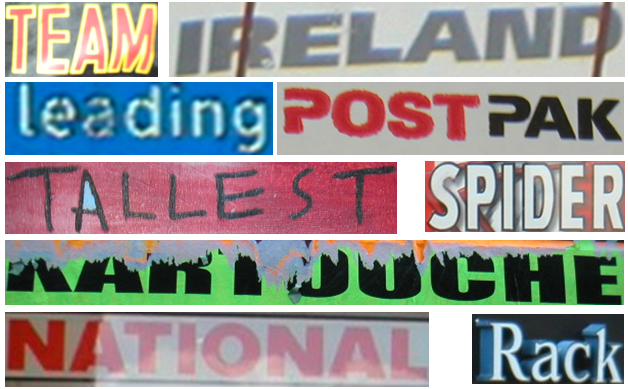
\includegraphics[scale=0.30]{img/cropped_words.png} }
		\caption[Reconocimiento de palabras recortadas]{Conjunto de palabras recortadas de diferentes escenas naturales. Imagen extraida del sitio de \textit{Graphics and Media Lab}, \url{http://graphics.cs.msu.ru/en/science/research/machinelearning/text}}
		\label{fig: Reconocimiento palabras}
	\end{figure}
		
	\end{itemize}

	Dada esta problemática, Wang et al. se enfocaron en un caso especial del reconocimiento de texto de escena donde tenían a disposición un listado de palabras (i.e, un lexicón) para detectar y leer.
		
	Para esto, ellos construyen y evalúan dos sistemas. En el primero, evalúan la performance en la detección y el reconocimiento de palabras de un enfoque con dos etapas que consiste en un detector de texto considerado estado del arte y un destacado motor de OCR. El segundo, es un sistema arraigado en el reconocimiento de objetos genéricos, el cual es una extensión de un trabajo que realizaron anteriormente \cite{WB10}. En \cite{WB10}, los autores consideran a las palabras como categorías de objectos en sí mismas y realizan reconocimiento sobre las categorías de las palabras. Utilizan técnicas propias del reconocimiento de categorías genéricas y las aplican al reconocimiento de palabras. Asi como podemos tener muchas imágenes que representen el objeto ``vehículo'', también es posible aplicar la misma idea para la palabra ``door'' como muestra la Figura \ref{fig: Reconocimiento generico}. La figura representa una analogía al reconocimiento de objetos genéricos.
	
	En \cite{wang}, los autores remarcan que para poder lograr el reconocimiento de palabras en imágenes, es necesario en primera instancia tener un clasificador de caracteres. Este trabajo se enfoca en el reconocimiento de caracteres en ventanas, es decir, imagenes de caracteres recortados de escenas naturales. 
	
	
	
	\begin{figure}[htbp]
		\centering
		\centerline{ 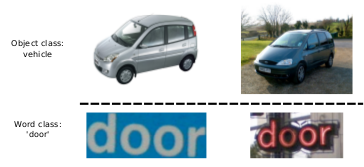
\includegraphics[scale=0.7]{img/object_recognition.png} }
		\caption[Reconocimiento generico de objetos]{Reconocimiento de palabras. Se considera a la palabra como una categoría de objeto al igual que la categoría ``vehiculo'' presentada en la parte superior de la imagen.}
		\label{fig: Reconocimiento generico}
	\end{figure}
	
	
	%\newpage
\subsection{Clasificación de imágenes naturales}

	\subsubsection{Características}

Las características en las imágenes naturales son muy variadas. Dentro de las mismas podemos encontrar las variaciones de intensidad en la iluminación, la resolución, el ángulo en el que son tomadas, el fondo, las texturas, entre otros. Mas específicamente, dependiendo del objeto que se esté analizando, por ejemplo, texto, surgen más características como el tipo de fuente, el tamaño, la posición y orientación de los caracteres, la contaminación que pueda llegar a tener el texto por suciedad u oclusión, etc. La infita variedad que es posible encontrar en este tipo de imágenes, dificultan el trabajo de reconocimiento sobre ellas por lo que, en general, es necesario realizar un pre-procesamiento antes de usarlas.

	En el caso del reconocimiento de texto, dada la gran cantidad de formas en que se puede encontrar la imagen de un carácter, es necesario encontrar algún método que extraiga las características mas representativas para poder distinguilo. Para poder analizar los caracteres en las imágenes naturales, uno de los enfoques que adoptan Wang et al. en \cite{wang} es el de trabajar con el descriptor HOG de cada imagen. Para poder entender que es un descriptor HOG (que se detalla en \ref{subsection:hog}), primero es necesario comprender el concepto de gradiente que se explica a continuación.
	
	%\paragraph{Imágenes naturales} ~\\

	\textbf{Cambiar el título}
	
	Las imágenes naturales siempre han sido un tema de interés en el campo de investigación de visión por computadora. La cantidad de información que puede proveer una imagen es gigantesca y la necesidad de poder procesar y reconocer es información ha llevado a los investigadores a proponer métodos para poder procesarla.	Aparte del puro interés científico, la popularidad se debe a la cantidad de aplicaciones prácticas que tiene el tema. Uno de los ejemplos más claros es el reconocimiento de patentes o LPR(por sus siglas en inglés)~\cite{DAB}, o el reconomiento de personas~\cite{DT05}, entre otros; sin embargo, no es una tarea sencilla ya que las imágenes naturales tienen infinitas variaciones que hacen díficil el reconomiento de objetos dentro de ellas.
	
	
	\subparagraph{Características} ~\\
	
		Las características en las imágenes naturales son muy variadas. Todas estas variaciones dificultan el trabajo sobre ellas por lo cual en general es necesario realizar un trabajo de pre-procesamiento antes de trabajar con las mismas. Las características que podemos encontrar en este tipo de imágenes son las variaciones de intensidad en la iluminación, la resolución, el ángulo en el que son tomadas las mismas, el fondo, las texturas, entre otros. Mas específicamente, dependiendo del objeto que se esté analizando, por ejemplo, texto en imágenes naturales, surgen más características como el tipo de fuente, el tamaño, la posición y orientación de los caracteres en el texto, la contaminación que pueda llegar a tener el texto por suciedad u oclusión, etc.
	
\paragraph{Gradientes} ~\\

	Sea $f(x_1,\dots,x_n)$ una función escalar de múltiples variables. El gradiente de $f$ representa la pendiente de la tangente del gráfico de $f$.  Mas precisamente, el gradiente apunta en la dirección donde se registra la mayor tasa de incremento de la función $f$ y su magnitud es la pendiente del gráfico de $f$ en esa dirección. Formalmente, es la generalización del concepto de derivada en funciones de múltiples variables.
		
	El gradiente de la función $f$ descripta anteriormente, es denotado como $\nabla f$ donde $\nabla$(el símbolo nabla) denota el operador diferencial. El gradiente de $f$ es definido como el único campo vectorial cuyo producto punto con cualquier vector $v$ en cada punto $x$ es la derivada direccional de $f$ a lo largo de $v$. Es decir,
		 \begin{align*}
		 	(\nabla f(x))\cdot v = D_v f(x)
		 \end{align*}
		 
	En un sistema de coordenadas rectangular, el gradiente es el campo vectorial cuyos componentes son las derivadas parciales de $f$:
		 
		 \begin{align*}
		 	\nabla f(x) = \frac{\partial f}{\partial x_1}\mathbf{e}_1 + \cdots + \frac{\partial f}{\partial x_n }\mathbf{e}_n
		 \end{align*}
	donde los $\mathbf{e}_i$ son vectores unitarios ortogonales que apuntan en la dirección de coordenadas.

	En el procesamiento de imágenes, un gradiente es un cambio direccional en la intensidad o color de la imagen. El vector gradiente se forma combinando la derivada parcial de la imagen en las direcciones $x$ e $y$. Se puede expresar del a siguiente forma:
		\begin{align}
			\nabla I = \left( \frac{\partial I}{\partial x} , \frac{\partial I}{\partial y} \right)
		\end{align}	
		
	Cuando determinamos la derivada parcial de $I$ respecto de $x$, determinamos la rapidez con que la imagen cambia de intensidad a medida que $x$ cambia. Para funciones continuas, $I(x,y)$, podemos expresarlo de la siguiente manera:
	\begin{align}
		\frac{\partial I(x,y)}{\partial x} = \lim_{\nabla x\rightarrow 0} \frac{I(x + \nabla x, y) - I(x,y)}{\nabla x}	
	\end{align}
	
	 El calculo de los gradientes de una imagen es útil ya que sirve, por ejemplo, para realizar detección de bordes de un objeto. En este caso, después de que los gradientes han sido computados, los píxeles con alto valor de gradiente son elegido como posibles bordes. Los píxeles con el valor de gradiente más alto en la dirección del gradiente se convierten en píxeles de borde. Los gradientes, también pueden ser usados en aplicaciones que realizan reconocimiento de objetos o correspondencia de texturas \textbf{agregar referencias}.

	
\subsubsection{Gradientes}
\label{subsubsection: Gradientes}

Sea $f(x_1,\dots,x_n)$ una función escalar de múltiples variables. Como expresa Gonzales et. al. en \cite{GonWoods}, el gradiente de $f$ es un vector que apunta en la dirección donde se registra la mayor tasa de incremento de la función. Su magnitud es la pendiente del gráfico en esa dirección. Es la generalización del concepto de derivada en funciones de múltiples variables.
		
	El gradiente de la función $f$ descrita anteriormente, es denotado como $\nabla f$ donde $\nabla$ (el símbolo nabla) denota el operador diferencial. El gradiente de $f$ es definido como el único campo vectorial cuyo producto punto con cualquier vector $v$ en cada punto $x$ es la derivada direccional de $f$ a lo largo de $v$. Es decir,
		 \begin{align*}
		 	(\nabla f(x))\cdot v = D_v f(x)
		 \end{align*}
		 
	En un sistema de coordenadas rectangular, el gradiente es el campo vectorial cuyos componentes son las derivadas parciales de $f$:
		 
		 \begin{align*}
		 	\nabla f(x) = \frac{\partial f}{\partial x_1}\mathbf{e}_1 + \cdots + \frac{\partial f}{\partial x_n }\mathbf{e}_n
		 \end{align*}
	donde los $\mathbf{e}_i$ son vectores unitarios ortogonales que apuntan en la dirección de coordenadas.

	En el procesamiento de imágenes, un gradiente es un cambio direccional en la intensidad o color de la imagen. En \cite{DJacobs}, Jacobs explica que el vector gradiente se forma combinando la derivada parcial de la imagen en las direcciones $x$ e $y$. Se puede expresar del a siguiente forma:
		\begin{align}
			\nabla I = \left( \frac{\partial I}{\partial x} , \frac{\partial I}{\partial y} \right)
		\end{align}	
		
	donde \textit{I}: $\mathbb{R}^{2} \rightarrow [0, 1]$ es la ``función intensidad'' que asigna un valor de intensidad a cada pixel (par (x,y)) de la imagen. Según Jacobs, cuando determinamos la derivada parcial de $I$ respecto de $x$, determinamos la rapidez con que la imagen cambia de intensidad a medida que $x$ cambia. Para funciones continuas, $I(x,y)$, podemos expresarlo de la siguiente manera:
	\begin{align}
		\frac{\partial I(x,y)}{\partial x} = \lim_{\nabla x\rightarrow 0} \frac{I(x + \nabla x, y) - I(x,y)}{\nabla x}	
	\end{align}
	
	 El cálculo de los gradientes de una imagen es útil ya que sirve, por ejemplo, para realizar detección de bordes de un objeto. La detección de bordes busca identificar puntos en una imagen en donde el brillo de la misma cambie de manera abrupta o, más formalmente, tenga discontinuidades. El propósito de esto es capturar eventos importantes o cambios en las propiedades de una imagen. En este caso, después de que los gradientes han sido computados, los píxeles con alto valor de gradiente son elegido como posibles bordes. Los píxeles con el valor de gradiente más alto en la dirección del gradiente se convierten en píxeles de borde. Los gradientes, también pueden ser usados en aplicaciones que realizan reconocimiento de objetos o correspondencia de texturas.	 
	
	\subsubsection{Características locales}

		\paragraph{Descriptor SIFT} ~\\

	\textit{Scale-invariant feature transform} o SIFT (por su sigla en inglés) es un algoritmo en visión por computadora desarrollado por David G. Lowe \cite{LoweDavid04} para detectar y describir las características locales de una imagen. Estas características, como se explico en secciones anteriores, sirven para identificar a una clase de interés u objeto cuando se la trata de localizar dentro de una imagen donde hay varios objetos. Los descriptores SIFT tienen la característica de no alterarse ante un cambio en la escala o en la orientación y son robustos en el sentido de que pueden detectar objetos si estos están desordenados o si los mismos están parcialmente ocultos. Además, son parcialmente invariantes a las transformaciones afines y a los cambios en la iluminación.
		
	Para obtener estas características, se realiza un muestreo de las orientaciones y magnitudes del gradiente de la imagen. En el trabajo de Lowe, este muestreo se realiza sobre regiones de $16 \times 16$ alrededor del punto de interés. Se analizan las muestras de cada región de $16 \times 16$ formando histogramas de orientaciones resumiendo el contenido en sub-regiones de $4 \times 4$. Cada uno de los histogramas se compone de 8 orientaciones. Por lo tanto se obtienen 16 histogramas respecto de las orientaciones de los puntos de cada región para cada uno de los puntos de interés. Finalmente el descriptor de cada punto de interés está formado por un vector que contiene los valores de las 8 orientaciones de los $4 \times 4$ histogramas, con lo cual se obtendría un vector de 128 elementos.

	Dado que los cambios en la iluminación afectan en mayor medida a la magnitud del gradiente y no a la orientación, se busca una representación de esta magnitud que minimice estos efectos. El objetivo es modificar al vector para darle cierta robustez frente a cambios en la iluminación. Para eso se lleva a cabo un proceso de normalización, donde los cambios en la luminosidad no afecta a los valores del gradiente. Finalmente, se limita el valor de cada componente de magnitud de gradiente a un valir máximo para que tenga un mayor peso la orientación frente a la magnitud del gradiente. Siguiendo los parámetros de Lowe en \cite{LoweDavid04}, el valor del umbral es de 0,2. Luego se vuelve a normalizar a una amplitud de unidad.

	
		
	
		\paragraph{Histograma de gradientes orientados} ~\\
\label{subsection:hog}

	Histograma de Gradientes Orientados o HOG (por sus siglas en inglés), son descriptores de características utilizados en visión por computadora y en el procesamiento de imágenes con el objetivo de realizar detección de objetos. Fueron introducidos por N. Dalal y B. Triggs en~\cite{DT05} con el propósito de realizar detección de personas; sin embargo, su uso no se limita solamente a esa área, sino que pueden ser utilizados en otras áreas como la detección de caracteres tal y como hizo Wang et al. en \cite{wang}.
	
	Todas las imágenes, como por ejemplo la presentada en la figura~\ref{fig: Imagen Letra original}, contienen objetos locales cuyas apariencias y formas pueden ser descriptas por la distribución de los gradientes de intensidad como se puede observar en la figura~\ref{fig: Image HOG}.	Un descriptor HOG, es un vector compuesto por una combinación de histogramas que representan los gradientes de intesidad en distintas regiones de una imagen. La implementación de estos descriptores, se obtiene dividiendo a la imagen en regiones de tamaño fijo llamadas celdas como se puede observar en la figura~\ref{fig: Image HOG celdas} y posteriormente, por cada celda, se calcula un histograma de gradientes para los píxeles en la celda ~\ref{fig: Cell Histogram}. Finalmente, como se explico anteriormente, el descriptor se obtiene de combinar los histogramas obtenidos~\ref{fig: Vector HOG}. La precisión se puede incrementar si se normalizan los histogramas, es decir, si se calcula una medida de la intensidad en una región más grande de la imagen, denominada bloque y se utiliza dicho valor para normalizar las celdas contenidas en el bloque.
	
	%El descriptor HOG mantiene una cuantas ventajas con respecto a otros métodos descriptores. Dado que el descriptor HOG opera en celdas localizadas, el método mantiene la invarianza a transformaciones geométricas y fotométricas, excepto para la orientación de objetos. Dichos cambios sólo aparecerían en regiones espaciales grandes~\cite{DT05}.
	
	En el área de visión por computadora, los descriptores HOG son considerados estado del arte o \textit{state of the art} al igual que muchos otros descriptores como \textit{SIFT}, \textit{Geometric Blur}, \textit{Shape Context}, \textit{Patch descriptor}, \textit{Maximum Response of filters} y \textit{Spin image}. Los descriptores HOG, han demostrado ser útiles en la clasificación como se puede apreciar en el trabajo de Wang et al.~\cite{wang} donde se ha entrenado el clasificador Random Ferns con estos. Incluso, se puede decir que la performance obtenida con estos descriptores en dicho trabajo supera a la mayoría de los descriptores evaluados en el trabajo de De Campos et al.~\cite{dCBV09} bajo las mismas condiciones de entrenamiento. Si bien Wang et al. usan como clasificador a Random Ferns y De Campos et al. usan en su evaluación SVM, se puede apreciar en la clasificación el impacto positivo al utilizar los descriptores HOG.
	
	La binarización de los descriptores HOG es necesaria, ya que las características binarias son fáciles de computar, son compactas, se pueden almacenar fácilmente y son fáciles de comparar. En cambio, los descriptores originales tienen alta dimensionalidad y requieren sistemas con más memoria, capacidad de almacenamiento y procesamiento. Uno de los beneficios de este enfoque en la clasificación, es que escala bien con la cantidad de categorías o clases. Muchos sistemas en tiempo real como el reconocimiento de objetos~\cite{SJC08} y en el agrupamiento de puntos clave~\cite{OFL07} han incorporado este enfoque por su utilidad.

	
	\paragraph{Binarización} ~\\

		A continuación se explicará un método para la binarización de los descriptores HOG. Para binarizar es necesario calcular un vector umbral. El umbral se calcula de la siguiente manera:
		\begin{itemize}
			\item Dado $N$ descriptores HOG de dimension $D$, se forma una matriz de tamaño $N \times D$ donde cada fila representa un vector.
			\item Se seleccionan $X$ columnas al azar de la matriz con reemplazo.
			\item Respetando el orden en que fueron seleccionadas, se aplica una función sobre cada columna (la función puede ser el calculo de la mediana, la media, bootstrap, entre otros), obteniendo de esta manera un vector nuevo $W$ de dimensión $X$ tal que cada dimensión de $W$ está compuesta por un par $(z,y)$ donde $y$ es un número talque $0 \leq y \leq D$ que representa una de las columnas elegidas de la matriz y $z$ representa el valor resultante de haber aplicado la función elegida a dicha columna. Cabe aclarar que $X$ puede ser mayor o menor a $D$ por lo cual el umbral $W$ puede tener mayor o menor dimensión al final.
		\end{itemize}
		Posteriormente dicho umbral $W$ se utiliza para binarizar los vectores originales de manera sencilla: sea $v_j$ con $j \in \{1,\dots,N\}$ uno de los $N$ vectores originales y tal que $v_j = d_1,d_2,\dots,d_D$. Luego se compara cada dimensión del umbral $W$ con la $y$-esima dimensión del vector $v_j$. Si $d_y \leq z$ se asigna 0, caso contrario 1. De esta manera binarizamos el vector $v_j$ obteniendo un nuevo vector binario de dimensión $X$.

		\begin{figure}[htbp]
			\centering
			\subfloat[Imagen original\label{fig: Imagen Letra original}]{
				\fbox{ 
\includegraphics[scale=0.3]{img/letter_A.jpg} }
			}
			\subfloat[Descriptores HOG de la imagen original\label{fig: Image HOG}]{
				\fbox{ 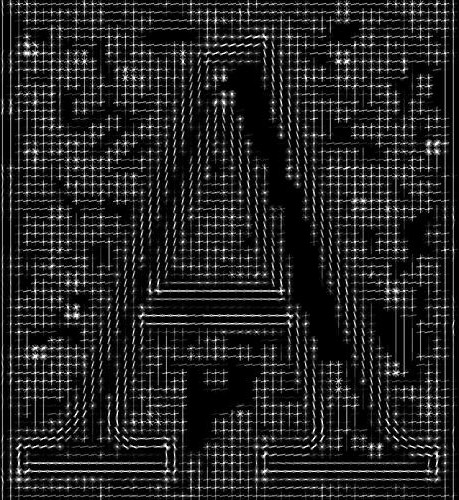
\includegraphics[scale=0.3]{img/letter_A_HOG.jpg} }
			}
			\\
			\subfloat[División por bloques de tamaño 4x4 celdas\label{fig: Image HOG celdas}]{
				\fbox{ 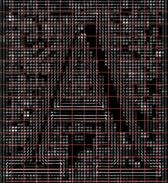
\includegraphics[scale=0.6]{img/letter_A_with_cells_2.jpg} }
			}
			\subfloat[Histograma de una celda\label{fig: Cell Histogram}]{
				\fbox{ 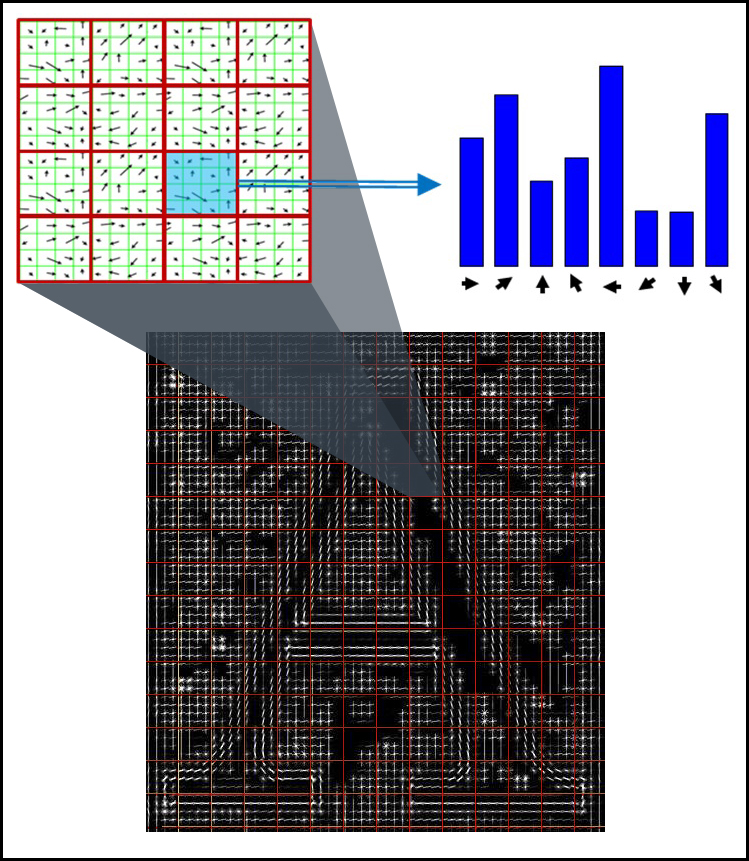
\includegraphics[scale=1.5]{img/letter_A_histogram.jpg} }
			}
			\caption{Descriptores HOG de la imagen de un caracter}
			\label{fig: HOG features}
		\end{figure}	

		\begin{figure}[htbp]
			\centering
			\fbox{ 
\includegraphics[scale=1]{img/feature_vector.jpg} }
			\caption[Vector HOG]{Formación del vector de características a partir de la concatenación de los histogramas. \textbf{CAMBIAR IMAGEN por algo mejor}}
			\label{fig: Vector HOG}
		\end{figure}

	
	\subsubsection{Reconocimiento de objetos}

	
	\subsection{Reconocimiento de caracteres}

	\begin{itemize}
		\item Algoritmos usados
			\begin{itemize}
				\item Introducción a Random Ferns: explicar el algoritmo y porqué lo usaron.
				\item HOG: hacer una ligera mensión de su uso. Los detalles van a estar en la sección correspondiente en el capítulo 2.
				\item non-maximal suppression (NMS) \JS{esto
                                    está asociado a esquemas de detección del tipo
                                    ``sliding window''}
			\end{itemize}
		\item Datasets usados \JS{no pondría nada sobre datasets acá,
                    sino mas bien una discusión sobre la necesidad de usar
                    datasets grandes para cubrir la variabilidad de apariencias
                  que aparecen en img reales}
			\begin{itemize}
				\item Aca puede ir una explicación del uso de datos sintéticos.
			\end{itemize}
	\end{itemize}
	
	%\subsection{Reconocimiento de palabras}
	\begin{itemize}
		\item Introducción a Pictorial Structures (Teoría)
		\item Uso de PS + Lexicón
		\begin{itemize}
			\item Algoritmo PLEX
		\end{itemize}
		\item Re-scoring y NMS
		\begin{itemize}
			\item Problemas con PLEX
		\end{itemize}
		\item Implementación
	\end{itemize}
	
	Para detectar palabras en una imagen, uno de los métodos que usan Wang et al., son las \textit{estructuras pictóricas} (\textit{pictorial structures}, de su traducción al inglés). Este enfoque toma las ubicaciones y puntajes de los caracteres detectados como entrada y encuentra la configuración óptima de una palabra específica. Formalmente, dada una palabra $w=(c_1,\dots , c_n)$ de $n$ caracteres de un lexicó, sea $L_i$ el conjunto de ubicaciones detectadas para el $i$-esimo carácter de $w$, y $u(l_i, c_i)$ sea puntuación de una detección particular en la ubicación $l_i \in L_i$ (obtenida a través del clasificador Random Ferns). La idea de este método, como ya se dijo, es obtener una configuración óptica $L^{*}=(l_1^{*}, \dots, l_n{*})$ optimizando la siguiente función:
	\begin{align}
		L^{*} = \underset{\forall i, l_i\in L_i}{argmin}\left( \sum_{i=1}^n -u(l_i, c_i) + \sum_{i=1}^{n-1} d(l_i,l_{i+1}) \right)
	\end{align}		
	
	donde $d(l_i, l_j)$ es el costo asociado de incorporar disposición espacial y similitud de escala entre dos caracteres vecinos. Usando programación dinámica se puede optimizar la ecuación anterior. Sea $D(l_i)$ el costo de colocación óptima de los caracteres $i+1$ a $n$ con la ubicación del $i$-esimo carácter fijado en $l_i$:
	\begin{align}
		D(l_i) = -u(l_i,c_i) + \underset{l_{i+1}\in L_{i+1}}{min} d(l_i,l_{i+1}) + D(l_{i+1})
	\end{align}
	Dada la naturaleza recursiva de $D(\cdot)$ se puede encontrar la configuración óptima pre-computando $D(l_n) = -u(l_n,c_n)$ para cada $l_n \in L_n$ y posteriormente trabajando para atrás hacia la primera letra.
	
	Una forma de extender dicha configuración para obtener las configuraciones de múltiples palabras, consiste en el uso de un algoritmo desarrollado por los autores denominado \textit{PLEX}. Consideremos el siguiente ejemplo, extraido del trabajo de Wang et al., el cual refleja muy bien el procedimiento. Supongamos que tenemos dos palabras en nuestro lexicón $\{$``ICCV'', ``ECCV'' $\}$. El valor de $D(l_2)$ es el mismo pues ambas palabras comparte el mismo sufijo ``CCV'', y por lo tanto puede ser computado una sola vez y usado para ambas palabras. Con esta idea en mente, se construye un árbol a partir de un lexicón donde cada letra de cada palabra del lexicón conforma un nodo y, empezando desde la última letra de la palabra, cada letra subsiguiente se encuentra en nivel inferior del árbol hasta alcanzar la primera letra (representada por un nodo coloreado o marcado como el inicio de la palabra). Con este enfoque, aquellas palabras que compartan un mismo sufijo, van a compartir el mismo recorrido en el árbol hasta que se separan. Cabe aclarar que el nodo raiz se lo considera ``vacio'' por lo cual la última letra de cada palabra representa el primer nodo descendiente de la raiz. En el peor de los casos, cuando dos palabras en un lexicón no comparte un sufijo común, este método es equivalete a realizar la configuración de cada palabra por separado.
	
	Unos de los problemas que presenta \textit{PLEX}, es que los puntajes no son compatibles para palabras de diferente longitud. El problema más imporante sin embargo, es que la función objetivo de las estructuras pictóricas captura solamente relaciones de a pares e ignora las características globales de la configuración.
	
	Dado esto, la última etapa del pipeline es realizar \textit{non-maximal suppression} sobre todas las palabras detectadas, Esto con el objetivo de incorporar algo de información global en esta última parte. Para eso, se vuelve a puntuar cada palabra retornada por \textit{PLEX} utilizando un clasificador \textit{Support Vector Machine} (\textit{SVM} por sus siglas en inglés).

	\RC{Falta experimentos}	
	
	
	\subsection{Arquitectura del sistema}
\label{subsection:impl_propia}

	El enfoque del presente trabajo se centra en los problemas de reconocmiento de caracteres y el reconocimiento de palabras. En las próximas subsecciones, se procederá a explicar cuestiones de implementación que se tuvieron en cuenta al momento de resolver ambos problemas.

	\subsubsection{Reconocimiento de caracteres}
		\label{subsubsection:recon-caracteres}
	
	
	\paragraph{Pipeline de procesamiento} ~\\

			La implementación que se realizó en este trabajo, está basada en un pipeline similar al que realizaron Wang et al. que comprende dos instancias: la instancia de entrenamiento y la instancia de evaluación. La primera esta constituida por la generación de datos sintéticos que constituyen el conjunto de entrenamiento, la extracción de las características, la binarización y el entrenamiento del clasificador. La segunda instancia consiste en la evaluación del clasificador que abarca desde la extracción y binarización de las características del conjunto de prueba y posteriormente la evaluación del clasificador para cada una de estas. El pipeline se puede apreciar en la figura \ref{fig: Pipeline entrenamiento}.

			\begin{figure}[htbp]
				\centering
				\centerline{
					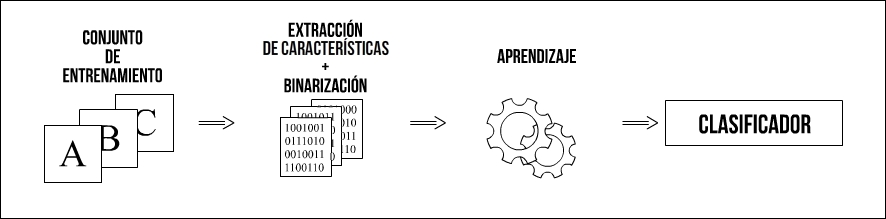
\includegraphics[scale=0.4]{img/pipeline_entrenamiento.jpg}
				}
				\caption[Pipeline de entrenamiento]{La figura representa el pipeline de entrenamiento que se sigue en el trabajo a la hora de entrenar el clasificador.}
				\label{fig: Pipeline entrenamiento}
			\end{figure}

		\paragraph{Conjunto de entrenamiento} ~\\
		
			La primera etapa de este pipeline de procesamiento es la obtención de un conjunto de entrenamiento que se va a utilizar para entrenar al clasificador por lo que es imporante tener una buena cantidad de imágenes ya que esto impacta en la performance de reconocimiento. Este trabajo hace uso del dataset \textit{Chars74k} \cite{dCBV09} del cual se generan todos los conjuntos de entrenamiento que se utilizan en los experimentos. Se destacan dos grupos de imágenes al momento de entrentar, el de  caracteres segmentados de escenas naturales y el de caracteres sintéticos. El primero viene incluido en el dataset nombrado, en cambio, el segundo, tiene que ser generado como se procederá a explicar a continuación.
			

		\paragraph{Generación de datos sintéticos} ~\\

			La datos sintéticos que se generan y utilizan en este trabajo son extraidos del dataset \textit{Chars74K} el cual está compuesto, entre otras cosas, por 62992 imágenes de caracteres sintéticos extraidos de fuentes de computadora. Cada una de las clases involucradas en la clasificación tienen un poco más de 1000 de estas imágenes (son 62 clases en total). El objetivo detrás de la generación de estos datos sintéticos es agregar vistas de los caracteres que no están reflejadas en el dataset original pero que son plausibles de ser observadas en la realidad.
			
			Inicialmente, se tiene como base un conjunto el cual contiene imágenes de caracteres de diversas fuentes. Lo que se busca, es aplicar a cada imagen un conjunto de transformaciones afines aleatorias con el objetivo final de obtener una imagen nueva con la apariencia  lo más cercana a una real. Una transformación afin consiste en una transformación lineal seguida de una traslación. Formalmente, cada transformación afín es de la forma $x\mapsto Mx + b$, donde $M$ es una transformación lineal y $b$ es un vector. Se usan las multiplicaciones entre matrices para representar las transformaciones lineales y la suma de vectores para representar las traslaciones. Mediante matrices ampliadas, sin embargo, es posible representar ambos tipos de transformaciones.	La matriz $M$ presentada anteriormente es una matriz $2\times 2$ y permite realizar transformaciones en imágenes de 2 dimensiones. En este trabajo, para generar los datos sintéticos se hacen uso de las siguientes transformaciones:
			
			\paragraph{Rotación}
			
				La rotación es una transformación afín que consta en rotar el ángulo de la imágen en el sentido anti-horario. El parámetro usado para el mismo son los radianes y las diferentes variaciones se pueden apreciar en la figura \ref{fig: Transformacion Afin - Rotacion}. Teniendo en cuenta la definición formal de una transformación afín anterior, la rotación formalmente se puede representar de la siguiente manera:

			\begin{equation*}
					M =  
					\begin{bmatrix}
						cos(\theta) & -sin(\theta) \\
						sin(\theta) & cos(\theta)  \\
					\end{bmatrix}
					b =
					\begin{bmatrix}
						0 \\
						0 \\
					\end{bmatrix}	
			\end{equation*}

	donde se puede observar el parámetros $\theta$ que representa el grado de inclinación y el vector $b$ es nulo por lo cual no hay traslación alguna.

		\begin{figure}[htbp]
			\centering
			\subfloat[\label{fig: sintetica original}]{
				\fbox{ 
\includegraphics[scale=1]{img/transformaciones/original.png} }
			}
			\subfloat[\label{fig: Imagen rad 0.5}]{
				\fbox{ 
\includegraphics[scale=1]{img/transformaciones/rotation0,5.png} }
			}
			\subfloat[\label{fig: Imagen rad 1}]{
				\fbox{ 
\includegraphics[scale=1]{img/transformaciones/rotation1.png} }
			}
			\subfloat[\label{fig: Imagen rad 1.5}]{
				\fbox{ 
\includegraphics[scale=1]{img/transformaciones/rotation1,5.png} }
			}
			\caption[Rotación de un caracter]{Rotación de un caracter. (a) Imagen original. (b) Imagen rotada 0.5 radianes. (c) Imagen rotada 1 radian. (d) Imagen rotada 1.5 radianes}
			\label{fig: Transformacion Afin - Rotacion}
		\end{figure}	
			
		\paragraph{Escala}
			
			La escala es una transformación que busca modificar el tamaño del objeto al cual se la aplica haciendola más chica o más grande lo que era originalmente. Formalmente, se puede representar por la siguiente configuración de la matriz $M$:
			\begin{equation}
				M = 
				\begin{bmatrix}
					a & 0 \\
					0 & d \\
				\end{bmatrix}
			\end{equation}
		donde $a$ y $d$ representan los cambios en los ejes $x$ e $y$ de la imagen respectivamente. Se puede apreciar la aplicación de esta transformación en la figura \ref{fig: Transformacion Afin - Escala}.
		\begin{figure}[htbp]
			\centering
			\subfloat[\label{fig: escala original}]{
				\fbox{ 
\includegraphics[scale=1]{img/transformaciones/original.png} }
			}
			\subfloat[\label{fig: Imagen escala 0.8}]{
				\fbox{ 
\includegraphics[scale=1]{img/transformaciones/scale0,8.png} }
			}
			\subfloat[\label{fig: Imagen escala 1.2}]{
				\fbox{ 
\includegraphics[scale=1]{img/transformaciones/scale1,2.png} }
			}
			\caption[Cambio de escala de un caracter]{Cambio de escala de un caracter. (a) Imagen original. (b) Imagen ampliada $1.2$ veces su tamaño  (c) Imagen reducida a $0.8$ veces su tamaño .}
			\label{fig: Transformacion Afin - Escala}
		\end{figure}	
			
		\paragraph{Transvección}
		
			La transvección es una transformación donde la imagen se rota en un solo eje. Es una función que toma un punto con coordenadas $(x,y)$ al punto $(x +ny, y)$ donde $n$ es un parámetro fijo, denominado el factor de inclinación. El efecto es el desplazamiento de todos los puntos horizontalmente en una cantidad proporcional a su coordenada $y$. Todo punto encima del eje $x$ es desplazado a la derecha si $n > 0$, y a la izquiera si $n < 0$. Nuestra matriz $M$ va a ser de la forma:
			\begin{equation}
				M = 
				\begin{bmatrix}
					1 & n \\
					0 & 1 \\
				\end{bmatrix}.
			\end{equation}
		Se puede observar en la figura \ref{fig: Transformacion Afin - Transveccion} los diferentes efectos de aplicar diferentes valores de $n$ en la aplicación de la transvección en una imagen.
		\begin{figure}[htbp]
			\centering
			\subfloat[\label{fig: Imagen transveccion 0.5}]{
				\fbox{ 
\includegraphics[scale=1]{img/transformaciones/shear0,5.png} }
			}
			\subfloat[\label{fig: Imagen transveccion 0.2}]{
				\fbox{ 
\includegraphics[scale=1]{img/transformaciones/shear0,20.png} }
			}
			\subfloat[\label{fig: Imagen original}]{
				\fbox{ 
\includegraphics[scale=1]{img/transformaciones/original.png} }
			}
			\subfloat[\label{fig: Imagen transveccion -0.2}]{
				\fbox{ 
\includegraphics[scale=1]{img/transformaciones/shear-0,20.png} }
			}
			\subfloat[\label{fig: Imagen transveccion -0.5}]{
				\fbox{ 
\includegraphics[scale=1]{img/transformaciones/shear-0,5.png} }
			}
			\caption[Transvección de un caracter]{Transvección de un carácter.}
			\label{fig: Transformacion Afin - Transveccion}
		\end{figure}	
		
		\paragraph{Traslación}		
			
			La traslación es el último tipo de transformación afín que usamos en este trabajo y a diferencia del resto de las transformaciones, esta no hace uso de $M$, sino de $b$ que es el vector de desplazamiento. Formalmente:
			\begin{equation*}
				M =  
					\begin{bmatrix}
						1 & 0 \\
						0 & 1  \\
					\end{bmatrix}
					b =
					\begin{bmatrix}
						b_1 \\
						b_2 \\
					\end{bmatrix}	
			\end{equation*}
		donde $b_1$ y $b_2$ representan el movimiento en el eje $x$ e $y$ respectivamente. Particularmente no usamos esta transformación para mover los caracteres, sino más bien para mantener la imagen del carácter centrada durante las diferentes transformaciones que le aplicamos a la imagen.
		
		\paragraph{Otras transformaciones:} ~\\
		\paragraph{Suavizado Gaussiano}
		
			Es una técnica que consta de la difuminación de una imagen a partir de la convolución con una función gaussiana. Se usa principalmente para reducir el ruido en una imagen. Dados das las coordenadas de un punto $(x, y)$ en una imagen, la función de suavizado es la siguiente
			\begin{align*}
				G(x,y) = \frac{1}{2\pi\sigma^2}\epsilon^{-\frac{x^2+y^2}{2\sigma^2}}
			\end{align*}
			donde $\sigma$ es la desviación estandard de la distribución gaussiana. En la figura \ref{fig: Suavizado Gaussiano}, se puede observar como distintos valores para $\sigma$ a medida que aumenta va distorcionando la imagen un poco más.
			
		\begin{figure}[htbp]
			\centering
			\subfloat[\label{fig: Imagen original sin blur	}]{
				\fbox{ 
\includegraphics[scale=1]{img/transformaciones/original.png} }
			}
			\subfloat[\label{fig: Imagen con blur 1}]{
				\fbox{ 
\includegraphics[scale=1]{img/transformaciones/blur1.png} }
			}
			\subfloat[\label{fig: Imagen con blur 2}]{
				\fbox{ 
\includegraphics[scale=1]{img/transformaciones/blur2.png} }
			}
			\caption[Suavizado Gaussiano de un caracter]{Aplicación de blur o suavizado gaussiano a un caracter. (a) Imagen original. (b) Imagen suavizada con un valor de $\sigma = 1$  (c) Imagen aún más suavizada con un valor de $\sigma = 2$ .}
			\label{fig: Suavizado Gaussiano}
		\end{figure}				
			
			
		\paragraph{Ruido Gaussiano}			
			
			El ruido en una imagen es una variación en la información sobre el color o la iluminación en la misma. Puede ser producido por un sensor, la circuitería de una escaner o una cámara digital. Condiciones de poca iluminación o interferencia electromagnética durante la transmisión de las imágenes son factores para que aparezca este tipo de distorsiones. El ruido gaussiano en las imágenes es un tipo de ruido que se caracteríza por tener una distribución gaussiana. La figura \ref{fig: Ruido Gaussiano} presenta 2 ejemplos de imágenes de caracteres con ruido gaussiano. A medida que el parámetro $\sigma$  aumenta, el ruido en la imagen se hace más notorio.
			
		\begin{figure}[htbp]
			\centering
			\subfloat[\label{fig: Imagen original sin ruido	}]{
				\fbox{ 
\includegraphics[scale=1]{img/transformaciones/original.png} }
			}
			\subfloat[\label{fig: Imagen con ruido 15}]{
				\fbox{ 
\includegraphics[scale=1]{img/transformaciones/noise15.png} }
			}
			\subfloat[\label{fig: Imagen con ruido 30}]{
				\fbox{ 
\includegraphics[scale=1]{img/transformaciones/noise30.png} }
			}
			\caption[Ruido Gaussiano en un caracter]{Aplicación de ruido gaussiano a un caracter. (a) Imagen original. (b) sigma=15  (c) sigma=30 .}
			\label{fig: Ruido Gaussiano}
		\end{figure}
			
			Un punto a destacar en este proceso, es que las fuentes de letras están en una escala de grises y se mantienen de esta forma. Esto es debido a que, durante el entrenamiento, solo es posible obtener las características de las imágenes sí y sólo sí estas están en escala de grises (requerimiento del algoritmo HOG). 
			
			
			%\paragraph{Anexar caracteres}
					
			%Otro tipo de modificación que vale la pena destacar, es la de anexar caracteres a los costados de la imagen a alterar. Esto es debido a que la mayoría de las imágenes de caracteres reales son extraidas de entornos donde la misma forma parte de una palabra. Es por eso que en la mayoría de los conjuntos generados, cada caracter está acompañado de pedazos de otros caracteres.
			
		%\begin{figure}[htbp]
		%	\centering
		%	\subfloat[\label{fig: Imagen anexo 1	}]{
		%		\fbox{ 
\includegraphics[scale=1]{img/transformaciones/anexo1.png} }
		%	}
		%	\subfloat[\label{fig: Imagen anexo 2}]{
		%		\fbox{ 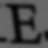
\includegraphics[scale=1]{img/transformaciones/anexo2.png} }
		%	}
		%	\subfloat[\label{fig: Imagen anexo 3}]{
		%		\fbox{ 
\includegraphics[scale=1]{img/transformaciones/anexo3.png} }
		%	}
		%	\caption[Caracteres pegados]{Imágenes de caracteres con caracteres pegados a izquierda y derecha.}
		%	\label{fig: Imagen anexos}
		%\end{figure}

		%	La creación de estos datos sintéticos son para el conjunto de entrenamiento del clasificador. El conjunto de test esta conformado por 15 imágenes reales por clase obtenidas del dataset \textit{Chars74K-15}, a las cuales no se les modifico en absoluto.

		\paragraph{Extracción de características y binarización} ~\\
		
			La siguiente etapa en el pipeline es la extracción del vector de características (ver sección ``Vectores de características'' \ref{subsection:feature}) de cada imagen del conjunto de entrenamiento y la binarización posterior de dicho descriptor (ver sección ``Binarización'' \ref{subsection:hog}).
			
			Una de las condiciones para poder extraer el vector de características de una imagen con HOG, es que esta esté en escala de grises o en blanco y negro. Luego, dado un conjunto de entrenamiento con $J$ imágenes, se construye una matriz $J \times K$ donde $K$ es la dimensión del descriptor HOG para cada imagen. Cabe aclarar que todas las imágenes tienen que tener las mismas dimensiones (48x48 píxeles) de lo contrario no se podría construir la matriz. Esto se debe a que HOG devuelve en sí un vector $v \in \mathbb{R}^{K}$ (donde $K$ depende de los parámetros que se le pasen al algoritmo y a la dimensión de la imagen). Posteriormente se procede como se detalla en \ref{subsection:hog} donde se obtiene el umbral que después se utiliza para binarizar todos los descriptores tanto del conjunto de entrenamiento como del conjunto de evaluación.
			
		

		\paragraph{Entrenamiento del clasificador}  ~\\

			En esta etapa, al igual que los autores del trabajo original, se utiliza como clasificador a Random Ferns. Para poder entrenar al clasificador, los vectores modificados de la etapa anterior se almacenan en un diccionario. Este último, esta estructurado como un conjunto de diccionarios anidados y representa la ``base de datos'' del sistema. Los detalles del porqué se eligió esta forma de almacenar la información se puede encontrar en el apéndice A. \RC{Crear apendice A donde se van a discutir cosas como lenguaje usado, base de datos, librerias entre otros}

			Dado que los vectores binarizados pertenecen al conjunto $\{ 0,1 \}^{N}$ si los quisiéramos almacenar en una sola tabla (habría una tabla por clase), cada una debería tener $2^{N}$ entradas lo cual si $N$ es muy grande sería imposible por la cantidad de memoria necesitada para mantener estas tablas en memoria. Luego, basándonos en lo explicado sobre Random Fern en \cite{subsection:ferns}, la solución pasa por dividir cada vector en $M$ grupos de dimensión $S = \frac{N}{M}$. Con esto, un vector completo esta almacenado en $M$ tablas diferentes (tablas correspondiente a la clase del vector). En total estaríamos trabajando con $M \times 62$ tablas (pues hay 62 clases diferentes).

			Dado un vector $v=(v_1, \dots, v_s)$ donde $v_i \in \{ 0,1 \}^{M}$, $z$ sea la clase de $v$ y sean $t_i i=1, \dots, s$ las tablas de $z$. Cada grupo $v_i i=1, \dots, s$ va a tener una entrada en su tabla correspondiente $z_i$ equivalente a su representación decimal. Inicialmente cada tabla está inicializada dado un parámetro $\alpha \neq 0$ que se explicará en detalle en el próximo capítulo.

		\paragraph{Evaluación del clasificador} ~\\

			Para la evaluación del clasificador, se toma como conjunto de test el descripto en la sección de descripción del dataset. A cada imágen del conjunto de test, se le extrae el descriptor HOG, se lo binariza y con el vector resultante se calcula la probabilidad de que dicho vector perteneza a cada una de las clases involucradas. El calculo para cada clase es el mismo y consiste en dividir el vector de prueba en $M$ grupos y por cada grupo obtener el valor en la tabla correspondiente. Por cada clase entonces tendríamos $M$ valores. Finalmente se realiza la suma de los logaritmos de cada valor y el resultado es la probabilidad de que ese vector pertenzca a la clase evaluada. Como es claro, al final se le asigna a la imagen evaluada la clase que haya obtenido la mayor probabilidad.


